\section{Across the mountains --- an unexperienced way to reach
Mig}

After two years with the ICCC, I finally made the decision to become a
Migovecer. Having done some cave exploration in Hungary, my idea of such
activities was spending endless hours of underground digging, in
passages of at most a 40 cm high, half-filled with dirty cold
water\ldots{}

Numbers better characterise these circumstances than words: in 10 years'
time, my Hungarian club made a steady progress of 400 m, the discovery
of almost every new meter being heavily aided by the products of the
HILTI company. Thus, \bignote{I was eagerly awaiting the Mecca of alpine-style
caving} and cave exploration. First, I spent a couple of days at a
Croatian-Hungarian caving expo, which had the double advantage of being
located next to the wonderful Zrmanja river, and to the local pub.

But after this wellness-spa holiday, I felt the urge to start true
caving, in the middle of the wilderness, on top of the unknown, mighty
\passage{Migovec}. So by hitch-hiking and a train journey, I arrived at \passage{Lake
Bohinj} to meet a friend and toss a day at the lake, after which I had
the illuminating idea of walking across the mountains instead of taking
public transportation to Tolmin and the going up from there.

According to my plans and my speed estimates, the trip could be made in
a day's time if one started early, thus even saving time compared to the
train journey! Thus, early in the morning, I started my ascent up to \passage{Dom
na Komni}. This path does endless hairpins up to the plateau, and no
wonder, I soon realised that the progress was much slower than
anticipated. Inexperienced in the Migovec conditions, I packed up well:
a complete cooking kit, various layers of clothing, and even some rope
completed the filling of my backpack and a large tackle-sack, which
altogether weighed about 30 kg's, not counting my secret meat stash
weighing a couple of kilos (which became sort of a tradition since
then), so I truly felt like a soldier of the first world war.

By the time I reached the hut, it was clear that the night will be spent
by bivouacking (as the money possibly spent for the hut fees was rather
spent on beer). So I made (or rather struggled) my way to the former
military camp, and set up my sleeping bag in the bushes, my torn poncho
being the only protection against rain - but why would it rain anyway in
such a wonderful, starry night, without a single cloud being visible,
and a wonderful weather forecast for the coming week?


\begin{marginfigure}
\checkoddpage \ifoddpage \forcerectofloat \else \forceversofloat \fi
\centering
 \frame{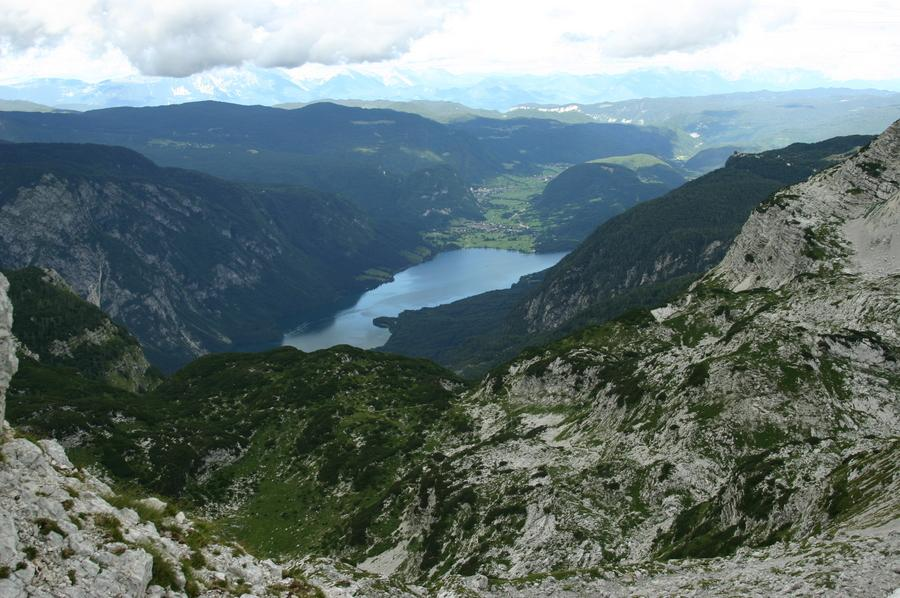
\includegraphics[width=\linewidth]{2008/across_mountains/Gergely Ambrus - DSLR - img_4933--orig.jpg}} 
 \caption{A view of \protect\passage{Lake Bohinj} \pic{Gergely Ambrus}}
 \label{bohinj gergely}
\end{marginfigure}


Having fallen asleep with such positive thoughts, my dream was
interrupted by a quite uncomfortable noise: thunder! The situation was
not welcoming, and at this moment I was not quite sure anymore whether
it was a good idea to liquidate my accommodation fees\ldots{}

However, a speedy action was needed, and luckily, I discovered a small
black hole next to the bushes. A cave! I imagined my first cave
exploration on Mig a bit differently, but here it was - speedily, I
managed to remove a couple of rocks blocking the entrance, and enlarged
the hole so that it could fit at least my packs plus half of me, the
other half covered by the torn poncho.

Of course, I hoped for a bit bigger, maybe down to -1000, but for the
moment being, this was sufficient enough to survive the storm - which
job it did at an agreeable level. It was neither dry nor comfortable,
but at least it gave the feeling of some protection against the
thunders, which hit the bushes around me in an alarming frequency.
Finally, the rain stopped, and it was time to recover my possessions,
and to start the remaining part of the journey.


\begin{marginfigure}
\checkoddpage \ifoddpage \forcerectofloat \else \forceversofloat \fi
\centering
 \frame{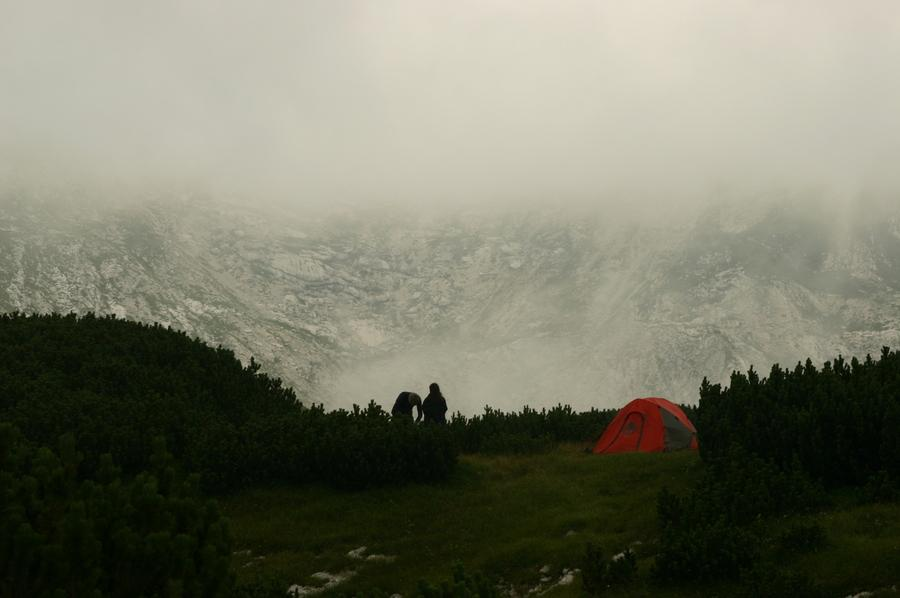
\includegraphics[width=\linewidth]{2008/across_mountains/Gergely Ambrus - DSLR - img_4835--orig.jpg}} 
 \caption{The plateau becomes increasingly difficult to navigate when the cloud comes down, particularly for cavers new to Migovec! \pic{Gergely Ambrus}}
 \label{plateau cloud gergely}
\end{marginfigure}



This was a bit complicated by the mist that now covered everything -
with about 10 m visibility, in the middle of the Northern plateau, with
way too much load, and finally, on the wrong side of \passage{Kuk}, it was
definitely not prospecting the most jolly day hike. Somehow I managed to
reach the saddle between \passage{Kuk} and \passage{Skrbina}, and from here, descended down
to the Migovec plateau following my compass bearings.

The task now was to find the bivvy, the only information of which was a
vaguely positioned red dot on my map (I didn't know about the magic
string then\ldots{}) So I wandered a bit up and down, and finally at the
edge of total exhaustion, surrounded by fog, a figure appeared on a rock
slab above me - a person with long hair, a long beard, barefoot and
wearing a long tunic - it could be nobody else, than Jesus!\sidenote{Although Jesus is the longstanding nickname of ICCC member Jan Evetts, on this occasion it was not he.}

At that moment, I realised that I never really imagined Heaven, but if I
did so by any means, the resulting scenery would definitely differ this
place. I also thought that it would be quite a hard task to collect all
my sins, adding to the final effort of crawling up the slope ahead of
me, by the time I meet Jesus\ldots{} Anyway, I made it to him, and I
gladly realised that the ghostly figure was a most real person: James
Huggett! Thus, my adventurous trip across the mountains has ended, and
soon I was welcomed by the other cavers, and had my first glimpse of the
ever-welcoming Bivvy.

\name{Gergely Ambrus}

\begin{figure*}[t!]
\checkoddpage \ifoddpage \forcerectofloat \else \forceversofloat \fi
\centering
    \begin{subfigure}[t]{0.393\textwidth}
        \centering
        \frame{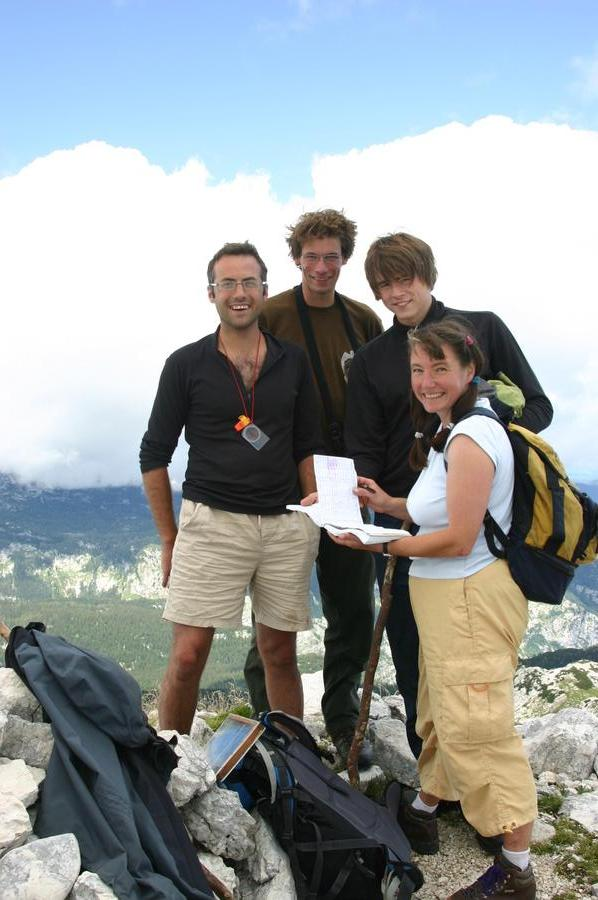
\includegraphics[width=\linewidth]{2008/across_mountains/Gergely Ambrus - DSLR - img_4903--orig.jpg}} 
        \caption{} \label{2008 group}
    \end{subfigure}
        \hfill
\begin{subfigure}[t]{0.59\textwidth}
\centering
\frame{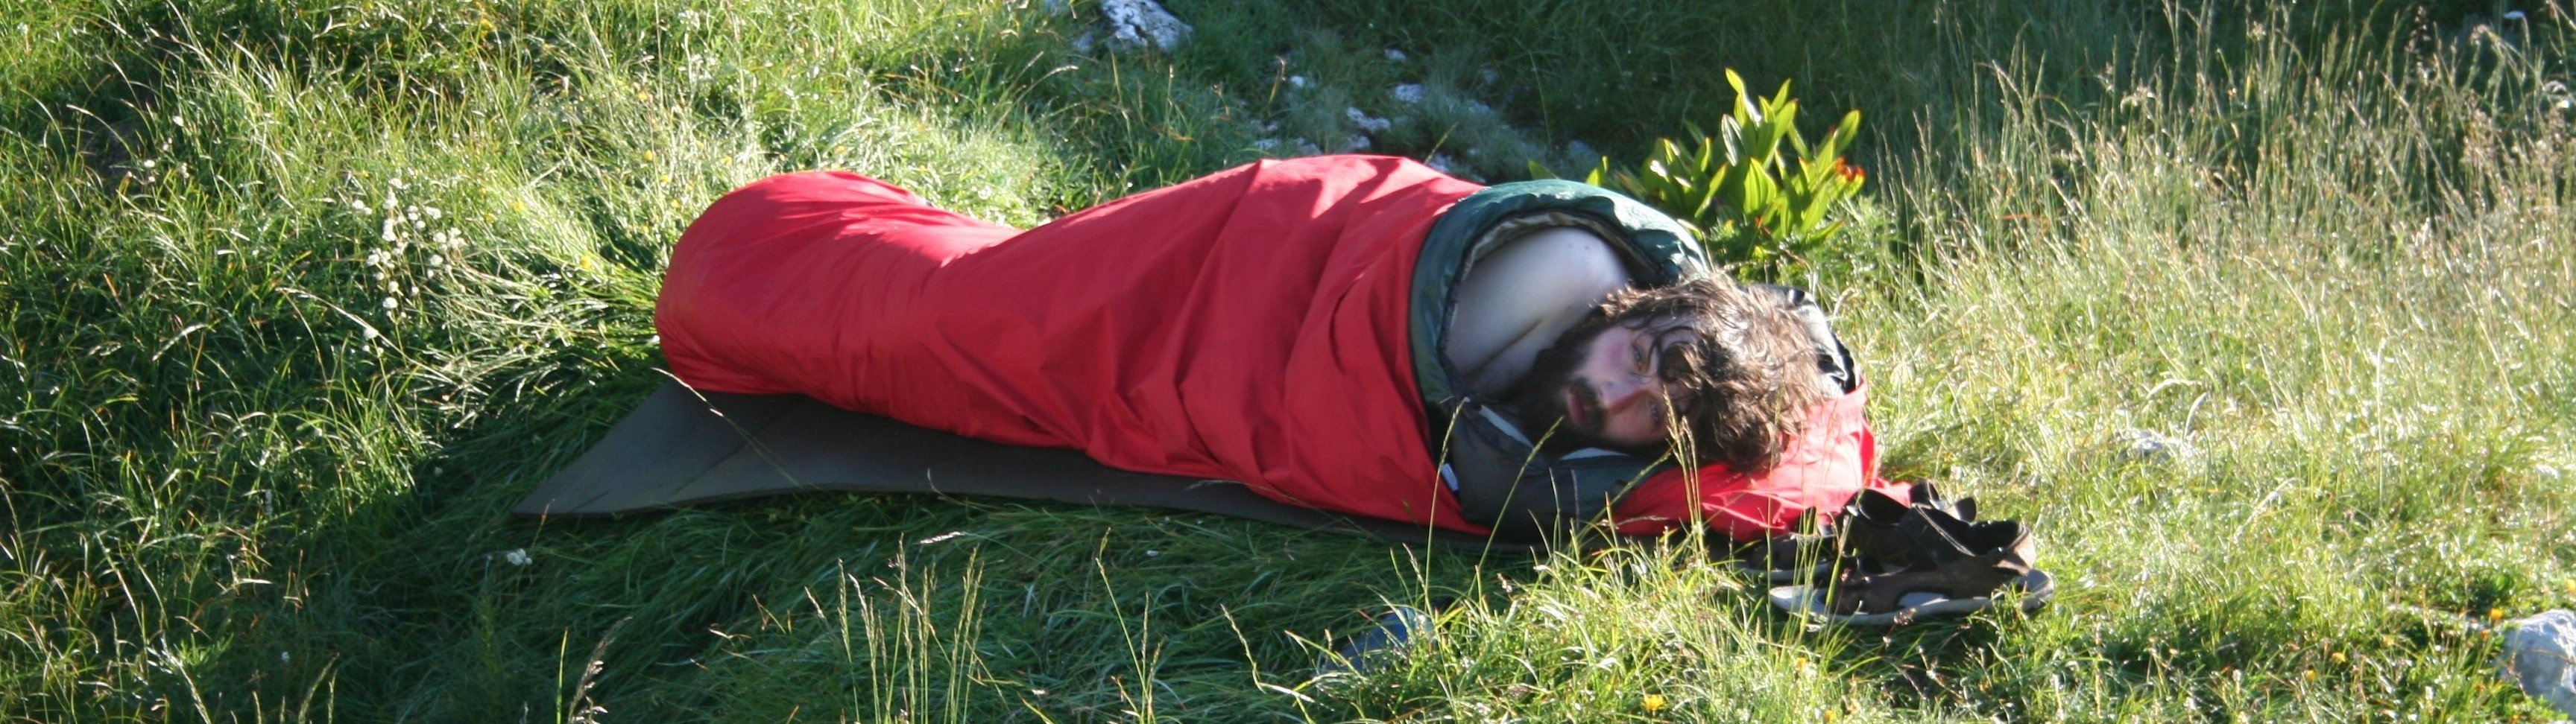
\includegraphics[width=\linewidth]{2008/across_mountains/Jana Carga - Canon 350D - img_3186 bivi bag on plateau James Huggett--orig.jpg}}
 \caption{}\label{fig:Huggy}
\end{subfigure}
    \caption{
    \emph{(a)} \emph{left to right} Tetley, Gergely Ambrus, Paul Hutton and Janet Cotter \pic{Gergely Ambrus}
     \emph{(b)} James Huggett \pic{Jana Carga} }
\end{figure*}
